Ολοκληρώνοντας τον κύκλο των δοκιμών για τους αλγορίθμους επιβλεπόμενης μάθησης, δημιουργήθηκε η ανάγκη για περαιτέρω έρευνα σε διαφορετικούς αλγορίθμους. Οι αλγόριθμοι επιβλεπόμενης μάθησης έχουν ένα βασικό μειονέκτημα, όταν προσεγγίζεται ένα πραγματικό πρόβλημα. Αυτό είναι η δυσκολίας εφαρμογής του αλγορίθμου, λόγω της έλλειψης των τάξεων των δεδομένων που απαιτεί ένα τέτοιο σύστημα για να εκπαιδευτεί. Η δυσκολία αυτή παρακάμπτεται χρησιμοποιώντας μη-επιβλεπόμενους ή ημι-επιβλεπόμενους αλγορίθμους που απαιτούν λίγα ή και κανένα ταξινομημένο παράδειγμα. Σε αυτό το κεφάλαιο θα προσεγγιστεί το πρόβλημα της ταξινόμησης καταναλωτών με νέα συστήματα που θα μπορούν να έχουν άμεσα χρήση στη λύση του πραγματικού προβλήματος, κάνοντας μια ανασκόπηση στις νέες δυσκολίες που προέκυψαν.
\section{Εξαγωγή Χαρακτηριστικών}
Στο παρόν μέρος θα γίνει παρουσίαση και ανάλυση των χαρακτηριστικών που χρησιμοποιήθηκαν στο μερικώς επιβλεπόμενο σύστημα, αλλά και στο μη επιβλεπόμενο σύστημα. Κάθε παράδειγμα μπορεί να περιγραφεί από ένα συνδιασμό τιμών που αναφέρονται επίσης ως μεταβλητές, χαρακτηριστικά, πεδία ή διαστάσεις. Οι τιμές αυτές μπορούν να είναι διαφορετικού τύπου όπως συνεχείς, δυαδικές ή κατηγορίες. Κάθε παράδειγμα μπορεί να αποτελείται μόνο από μια τιμή (μονοπαραγοντικό) ή και από περισσότερες (πολυπαραγοντική). Στην περίπτωση των πολυπαραγοντικών παραδειγμάτων, όλες οι τιμές μπορεί να είναι ίδιου τύπου ή μπορεί να είναι ένας συνδυασμός διαφορετικών τύπων \cite{Anomaly}.\\
Παράλληλα, κάθε παράδειγμα μπορεί να οριστεί βάση ακόμη δύο δομών ως προς τον ορισμό του προβλήματος \cite{Anomaly}.
\begin{enumerate}
\item{\textit{Τιμές Συσχετισμού}} Τέτοιου είδους τιμές χρησιμοποιούνται για να περιγράψουν ένα γενικό πλαίσιο που χαρακτηρίζει ένα παράδειγμα. Στις χρονοσειρές, ο χρόνος είναι μια τιμή που παρέχει μια σχετικότητα, η οποία καθορίζει τη θέση ενός παραδείγματος σε μια ολόκληρη ακολουθία. Μία τιμή γενικού πλαισίου είναι η μηνιαία κατανάλωση ενός κατοίκου.
\item{\textit{Συμπεριφορικές Τιμές}} Είναι οι τιμές που δεν προδίδουν ένα γενικό πλαίσιο για κάποιο παράδειγμα ή κάποια σχετικότητα. Ένα τέτοιο παράδειγμα θα μπορούσε να είναι η ετήσια παραγωγή ενέργειας σε όλο τον κόσμο.
\end{enumerate}
\subsection{Φύση Χαρακτηριστικών}
Το μερικώς επιβλεπόμενο και μη επιβλεπόμενο σύστημα απαιτούν εισόδους που να δίνουν τη δυνατότητα να διαχωρίζονται σε δύο κλάσεις οι καταναλωτές. Για να γίνει αυτό απαιτείται η χρήση χαρακτηριστικών που να αντιπροσωπεύουν την κλάση, αλλά και χαρακτηριστικά που προσδίνουν γενικότητα στο κάθε παράδειγμα. Με αυτό τον τρόπο παρέχεται ένα περιθώριο στον αλγόριθμο, έτσι ώστε να μπορεί εύκολα να προσαρμόζεται σε καινούργια και ξεχωριστά παραδείγματα. Ένας απλοϊκός τρόπος να διαχωρίσουμε τα χαρακτηριστικά είναι σε χαρακτηριστικά γενίκευσης και σε χαρακτηριστικά διαχωρισμού κλάσεων. Όλα τα παρακάτω χαρακτηριστικά αποτελούν τιμές συσχέτισης.
\subsubsection{Χαρακτηριστικά Γενίκευσης} 
Τα πλεονέκτημα των χαρακτηριστικών γενίκευσης είναι ότι βοηθούν στην κατάταξη του καταναλωτή σε σχέση με τους υπόλοιπους, ώστε να εξαχθούν πληροφορίες, όπως ο τύπος καταναλωτή (οικιακού ή βιομηχανικού) και το προφίλ κατανάλωσής του. Τέτοια χαρακτηριστικά πρέπει να περιορίζονται σε αριθμό όμως, καθώς ενδέχεται να δυσκολεύσουν τον διαχωρισμό με βάση το κριτήριο που θέτουμε παρέχοντας μεγάλο παράγοντα γενίκευσης.  Τέτοιου είδους χαρακτηριστικά είναι τα παρακάτω:
\begin{enumerate}
\item{\textit{Ετήσια μέση τιμή ημίωρου}} Βρίσκεται ο μέσος όρος ημίωρου κάθε μέρας και για όλες τις μέρες του έτους βρίσκεται ο ετήσιος μέσος όρος.
\item{\textit{Ετήσια τυπική απόκλιση ημίωρου}} Βρίσκεται η τυπική απόκλιση κάθε μέρας και για όλες τις μέρες του έτους βρίσκεται ο ετήσιος μέσος όρος της τυπικής απόκλισης.
\item{\textit{Διαφορά Ετήσιου Ελάχιστου τάσης με όμοιους}} Βάση αυτού του χαρακηριστικού ορίζεται για όμοιους καταναλωτές το ελάχιστο της τάσης κατανάλωσής τους και στην συνέχεια βρίσκεται η απόλυτη διαφορά σε  ημέρες.
\item{\textit{Διαφορά μέσης τιμής με ομοίους}} Με αυτό το χαρακτηριστικό βρίσκεται η διαφορά του ετήσιου μέσου όρου κάθε καταναλωτή με την ομάδα καταναλωτών που ανήκει.
\item{\textit{Διαφορά τυπικής απόκλισης με ομοίους}} Με αυτό το χαρακτηριστικό βρίσκεται η διαφορά της ετήσιας τυπικής απόκλισης κάθε καταναλωτή με την ομάδα καταναλωτών που ανήκει.
\end{enumerate}
\subsubsection{Χαρακτηριστικά Διαχωρισμού}
Τα χαρακτηριστικά διαχωρισμού επικεντρώνονται στην όξυνση των διαφορών μεταξύ των καταναλωτών διαφορετικών κλάσεων. Λειτουργούν, λοιπόν σαν οδηγοί για τον αλγόριθμο ώστε να κάνουν πιο εμφανείς τις διαφορές των κλάσεων. Το πλεονέκτημα τους είναι ο παράγοντας εξειδίκευσης που παρέχουν στον αλγόριθμο διευκολύνοντας τον να αναγνωρίζει με διαφορετικούς τρόπους κάθε κλάση. Το μειονέκτημα είναι πως λόγο της εξειδικευμένης τους φύσης μπορεί να μην εφαρμόζονται απόλυτα από όλους τους καταναλωτές ή στην χειρότερη περίπτωση να περιγράφουν μια σπάνια συμπεριφορά που δεν ενδιαφερόμαστε να διαχωρίσουμε.
\begin{enumerate}
\item{\textit{Κινούμενος μέσος όρος μηνιαίου μέσου όρου}} Πρόκειται για υπό συνθήκη χαρακτηριστικό που αν παρατηρήσει κάποια σημαντική πτώση των καταναλώσεων τότε ψάχνει για την μέγιστη και την καταγράφει. Ορίζοντας ως $min$ τον μήνα του ελαχίστου και $c$ την κατανάλωση του αντίστοιχου $i$ μήνα θα έχω την εξής φόρμουλα για αυτό το χαρακτηριστικό. 
\begin{center}
\resizebox{8cm}{!}{$\bar{c_{p}}-\bar{c_{a}}=\frac{1}{k-1}\sum_{i=1}^{k} c_{m-i}-\frac{1}{w}\sum_{i=0}^{w}  c_{m+i}$}
\end{center}
\item{\textit{Κινούμενος μέσος όρος μηνιαίας τυπικής απόκλισης}} Πρόκειται για υπό συνθήκη χαρακτηριστικό που αν παρατηρήσει κάποια σημαντική πτώση της τυπικής απόκλισης τότε ψάχνει για την μέγιστη και την καταγράφει. Ορίζοντας ως $min$ τον μήνα του ελαχίστου και $std$ την τυπική απόκλιση της κατανάλωσης τον αντίστοιχο $i$ μήνα θα έχω την εξής φόρμουλα για αυτό το χαρακτηριστικό. 
\begin{center}
\resizebox{8.8cm}{!}{$\bar{std_{p}}-\bar{std_{a}}=\frac{1}{k-1}\sum_{i=1}^{k} std_{m-i}-\frac{1}{w}\sum_{i=0}^{w}  std_{m+i}$}
\end{center}
\item{\textit{Συμμετρική διαφορά καταναλώσεων}} Πρόκειται για υπό συνθήκη χαρακτηριστικό που παρατηρεί μια γενική συμπεριφορά όμοιων καταναλωτών ως προς τη χρονική στιγμή της ελάχιστης κατανάλωσης και ψάχνει για κάποια σημαντική πτώση της κατανάλωσης ανάμεσα σε 2 συμμετρικές χρονικές στιγμές με άξονα συμμετρίας την εκάστοτε χρονική στιγμή ελαχίστου. Ορίζοντας ως $min$ την ημέρα του ελαχίστου και $c$ την κατανάλωση της αντίστοιχης $i$ ημέρα θα έχω τις εξής φόρμουλες εισάγοντας σε αυτό το σημείο και την ευκλείδεια απόσταση.
\begin{center}
\resizebox{8cm}{!}{$\bar{c_{p}}-\bar{c_{a}}=\frac{1}{n}\sum_{i=1}^{n+1} c_{min-i}-\frac{1}{n}\sum_{i=0}^{n}  c_{min+i}$}
\resizebox{9cm}{!}{$||c_{p}||-||c_{a}||=\sqrt{\sum_{i=1}^{n+1} (c_{min-i})^2}-\sqrt{\sum_{i=0}^{n}  (c_{min+i})^2}$}
\end{center}
\item{\textit{Συμμετρική διαφορά τυπικής απόκλισης}} Πρόκειται για υπό συνθήκη χαρακτηριστικό που παρατηρεί μια γενική συμπεριφορά όμοιων καταναλωτών ως προς τη χρονική στιγμή της ελάχιστης κατανάλωσης και ψάχνει για κάποια σημαντική πτώση της τυπικής απόκλισης ανάμεσα σε 2 συμμετρικές χρονικές στιγμές με άξονα συμμετρίας την εκάστοτε χρονική στιγμή ελαχίστου. Ορίζοντας ως $min$ την ημέρα του ελαχίστου και $std$ την την τυπική απόκλιση της κατανάλωσης την αντίστοιχη $i$ ημέρα θα έχω τις εξής φόρμουλα για αυτό το χαρακτηριστικό. 
\begin{center}
\resizebox{9cm}{!}{$\bar{std_{p}}-\bar{std_{a}}=\frac{1}{n}\sum_{i=1}^{n+1} std_{min-i}-\frac{1}{n}\sum_{i=0}^{n}  std_{min+i}$}
\resizebox{10cm}{!}{$||std_{p}||-||std_{a}||=\sqrt{\sum_{i=1}^{n+1} (std_{min-i})^2}-\sqrt{\sum_{i=0}^{n}  (std_{min+i})^2}$}
\end{center}
\item{\textit{Τμηματική διαφορά κατανάλωσης με όμοιους καταναλωτές}} Πρόκειται για υπό συνθήκη χαρακτηριστικό που παρατηρεί μια γενική συμπεριφορά όμοιων καταναλωτών ως προς τη χρονική στιγμή της ελάχιστης κατανάλωσης και ψάχνει για κάποια σημαντική πτώση της κατανάλωσης ανάμεσα στον καταναλωτή και τους όμοιούς του μετά την χρονική στιγμή της ελάχιστης κατανάλωσης. Πιο φορμαλιστικά θεωρώντας τους όρους $c_{cl}$ την τυπική κατανάλωση μιας ομάδας και $c_{co}$ την κατανάλωση ενός καταναλωτή έχουμε την παρακάτω διαφορά μέσων όρων και νορμών των καταναλώσεων.
\begin{center}
\resizebox{9cm}{!}{$\bar{c_{cl}}-\bar{c_{co}}=\frac{1}{n}\sum_{i=1}^{n+1} c_{cl,min-i}-\frac{1}{n}\sum_{i=0}^{n}  c_{co,min+i}$}
\resizebox{10cm}{!}{$||c_{cl}||-||c_{co}||=\sqrt{\sum_{i=1}^{n+1} (c_{cl,min-i})^2}-\sqrt{\sum_{i=0}^{n}  (c_{co,min+i})^2}$}
\end{center}
\item{\textit{Τμηματική διαφορά τυπικής απόκλισης με όμοιους καταναλωτές}} Πρόκειται για υπό συνθήκη χαρακτηριστικό που παρατηρεί μια γενική συμπεριφορά όμοιων καταναλωτών ως προς τη χρονική στιγμή της ελάχιστης κατανάλωσης και ψάχνει για κάποια σημαντική πτώση της τυπικής απόκλισης ανάμεσα στον καταναλωτή και τους όμοιούς του μετά την χρονική στιγμή της ελάχιστης κατανάλωσης. Πιο φορμαλιστικά θεωρώντας τους όρους $std_{cl}$ την τυπική κατανάλωση μιας ομάδας και $std_{co}$ την κατανάλωση ενός καταναλωτή έχουμε την παρακάτω διαφορά μέσων όρων και νορμών των τυπικών αποκλίσεων των καταναλώσεων.
\begin{center}
\resizebox{10cm}{!}{$\bar{std_{cl}}-\bar{std_{co}}=\frac{1}{n}\sum_{i=0}^{n}  std_{cl,min+i}-\frac{1}{n}\sum_{i=0}^{n}  std_{co,min+i}$}
\resizebox{11cm}{!}{$||std_{cl}||-||std_{co}||=\sqrt{\sum_{i=0}^{n} (std_{cl,min+i})^2}-\sqrt{\sum_{i=0}^{n}  (std_{co,min+i})^2}$}
\end{center}
\item{\textit{Χρονική Διαφορά Ελαχίστου}} Πρόκειται για υπό συνθήκη χαρακτηριστικό που εξερευνά το ελάχιστο χρονικό σημείο της τάσης της καμπύλης κάθε καταναλωτή. Με βάση την ομάδα που ανήκει κάθε καταναλωτής υπολογίζεται η απόλυτη τιμή της χρονικής διαφοράς μεταξύ του ελαχίστου κάθε καταναλωτή με την ομάδα που ανήκει. Χρησιμοποιώντας ένα όριο για τη διαφορά αυτή γίνεται αντιληπτή οποιαδήποτε έντονη διακύμανση του καταναλωτή με την ομάδα του και καταγράφεται σαν χαρακτηριστικό διαχωρισμού από την αναμενόμενη συμπεριφορά κατανάλωσης.
\begin{center}
\resizebox{3.5cm}{!}{$|t_{cl,min}-t_{co,min}|$}
\end{center}
\end{enumerate}

\subsection{Δοκιμή Χαρακτηριστικών με σταθερή απάτη}
Αφού οριστούν τα χαρακτηριστικά που εκτιμάται ότι μπορούν να βοηθήσουν στον διαχωρισμό των κλάσεων, έπεται φυσικά η δοκιμή τους με έναν αφελή τρόπο, έτσι ώστε να επιβεβαιωθεί ότι μπορούν να λειτουργήσουν όπως αναμένεται. Παράλληλα, η δοκιμή αυτή παρέχει μεγάλο όγκο πληροφορίας, αφού καθιστά εμφανή τα σημεία και τις προϋποθέσεις που τα χαρακτηριστικά έχουν μεγάλη ακρίβεια, αλλά και εκεί που υστερούν.

Ο κώδικας της δοκιμής θεωρεί δεδομένη και σταθερή την ένταση κλοπής και την ημέρα που κάθε καταναλωτής ξεκινά να αλλοιώνει τις τιμές του. Ειδικότερα, το ποσοστό των καταναλωτών που αλλοιώνει τις μετρήσεις του είναι 50 τοις εκατό, η ένταση της κλοπής είναι της τάξης του 80 τοις εκατό και η μέρα κλοπής ορίζεται η 182η, δηλαδή μετά από 6 μήνες κανονικής κατανάλωσης ο χρήστης εισάγει σύστημα αλλοίωσης της μέτρησής του. Δοκιμάζοντας ξεχωριστά τα χαρακτηριστικά διαχωρισμού ελέγχουμε το όριο κάθε χαρακτηριστικού έτσι ώστε να δώσει μεγαλύτερη ακρίβεια στις επιθέσεις δεδομένων υπό τις παραπάνω συνθήκες. Αν ο παρατηρηθούν τέτοια χαρακτηριστικά ο καταναλωτής θεωρείται θετικός στην κλοπή. Αντίθετα αν ο καταναλωτής δεν έχει την αναμενόμενη συμπεριφορά το χαρακτηριστικό δεν καταγράφει κάποια τιμή και ο καταναλωτής θεωρείται αρνητικός στην κλοπή. Αναλυτικότερα για κάθε χαρακτηριστικό διαχωρισμού λήφθηκαν τα παρακάτω αποτελέσματα:
\begin{enumerate}
\item{\textit{Κινούμενος μέσος όρος μηνιαίου μέσου όρου}} \\
Στην πρώτη δοκιμή δόθηκε έμφαση στη γενικότερη συμπεριφορά του χαρακτηριστικού ως προς το όριο που τίθεται κάθε φορά. Έτσι παρατηρείται εύκολα πως για μεγάλο όριο ο διαχωρισμός έχει χαμηλή ακρίβεια με εξαιρετικά μικρό ποσοστό αποτυχίας. Αντίθετα, αν το όριο χαμηλώσει αισθητά ο χάνεται η έννοια του διαχωρισμού και ο αλγόριθμος θεωρεί θετικούς σε κλοπές σχεδόν όλους τους καταναλωτές.
\begin{center}
\begin{tabu} to 0.8\textwidth { | X[c] || X[c] | X[c] | X[c] | X[c] | X[c] |  }
 \hline
 \multicolumn{6}{|c|}{Δοκιμή 1ου χαρακτηριστικού} \\
 \hline
  Όριο & \en{DR}  & \en{FPR} & \en{BDR} & \en{Accuracy} & \en{F1}\\
 \hline
 0,8&	44,8&	1,4	&0,97	&71,7&	61,29\\
0,7&	98,7&	1,9	&0,98	&98,4&	98,4\\
0,6&	99,3&	3,6&	0,97&	97,85&	97,88\\
0,5&	99,8&	7,5	&0,93	&96,15&	96,15\\
0&	99,9&	91,5	&0,52	&54,2&	68,57\\
\hline
\end{tabu}
\end{center}

\item{\textit{Κινούμενος μέσος όρος μηνιαίας τυπικής απόκλισης}} \\
Αντίστοιχα και εδώ για παρόμοιες τιμές του ορίου με το προηγούμενο χαρακτηριστικό ο διαχωρισμός είναι εξαιρετικά εύστοχος και δεν αφήνει περιθώρια για αμφισβήτηση.
\begin{center}
\begin{tabu} to 0.8\textwidth { | X[c] || X[c] | X[c] | X[c] | X[c] | X[c] |  }
 \hline
 \multicolumn{6}{|c|}{Δοκιμή 2ου χαρακτηριστικού} \\
 \hline
  Όριο & \en{DR}  & \en{FPR} & \en{BDR} & \en{Accuracy} & \en{F1}\\
 \hline
0,7	&98,2	&2,3	&0,98	&98,3	&98,31\\
0,6	&99,8	&4,1	&0,96	&97,85	&97,89\\
0,5	&99,5	&8,2	&0,92	&95,65	&95,81\\
\hline
\end{tabu}
\end{center}
\item{\textit{Συμμετρική διαφορά καταναλώσεων}} \\
Το συγκεκριμένο χαρακτηριστικό δεν δίνει αξιόπιστα αποτελέσματα, καθώς η συμμετρία που προκύπτει από τον χρησιμοποιούμενο τύπο απάτης κάνει το συγκεκριμένο χαρακτηριστικό να αποτυγχάνει σε αυτή τη δοκιμή. Παρόλα αυτά, το χαμηλό ποσοστό αποτυχίας αφήνει δεύτερες σκέψεις, καθώς δεν επιβαρύνει αισθητά τα αποτελέσματα, αλλά βοηθά στη γενίκευση του τύπου κλοπής. 
\begin{center}
\begin{tabu} to 0.8\textwidth { | X[c] || X[c] | X[c] | X[c] | X[c] | X[c] |  }
 \hline
 \multicolumn{6}{|c|}{Δοκιμή 3ου χαρακτηριστικού} \\
 \hline
  Όριο & \en{DR}  & \en{FPR} & \en{BDR} & \en{Accuracy} & \en{F1}\\
 \hline
 0,1&	26,3&	5,7&	0,82&	60,3&	39,85\\
\hline
\end{tabu}
\end{center}
Η δοκιμή συνεχίστηκε και με τις νόρμες των καταναλώσεων, παρατηρώντας ελάχιστη βελτίωση στο \en{DR}, ενώ αισθητά καλύτερα αποτελέσματα παρατηρούνται στο \en{FPR} που μειώθηκε ακόμη περισσότερο.
\begin{center}
\begin{tabu} to 0.8\textwidth { | X[c] || X[c] | X[c] | X[c] | X[c] | X[c] |  }
 \hline
 \multicolumn{6}{|c|}{Δοκιμή 3ου χαρακτηριστικού με νόρμες} \\
 \hline
  Όριο & \en{DR}  & \en{FPR} & \en{BDR} & \en{Accuracy} & \en{F1}\\
 \hline
 0,3&	29&	2,1&	0,93&	63,65&	44,71\\
\hline
\end{tabu}
\end{center}

\item{\textit{Συμμετρική διαφορά τυπικής απόκλισης}} \\
Αντίστοιχα συμπεράσματα ισχύουν και στη συμμετρική διαφορά τυπικής απόκλισης που οριακά ξεπερνά το 10 τοις εκατό στο \en{FPR}. Η γενίκευση που προσφέρει παρόλα αυτά το συγκεκριμένο χαρακτηριστικό είναι χρήσιμη, καθώς εν τέλει όλα τα χαρακτηριστικά θα ενώσουν τα δυνατά τους σημεία για να διαχωρίσουν απάτες με μεγαλύτερο τυχαίο παράγοντα.
\begin{center}
\begin{tabu} to 0.8\textwidth { | X[c] || X[c] | X[c] | X[c] | X[c] | X[c] |  }
 \hline
 \multicolumn{6}{|c|}{Δοκιμή 4ου χαρακτηριστικού} \\
 \hline
  Όριο & \en{DR}  & \en{FPR} & \en{BDR} & \en{Accuracy} & \en{F1}\\
 \hline
 0,1&	38,9&	10,2&	0,79&	64,35&	52,18 \\
\hline
\end{tabu}
\end{center}
Σε αυτό το σημείο η μείωση του \en{FPR} είναι αρκετά σημαντικό ζήτημα που τελικώς επιτεύχθει με τις νόρμες που μπόρεσαν να μειώσουν το \en{FPR} χωρίς να επηρεάσουν αρνητικά το \en{DR}. 
\begin{center}
\begin{tabu} to 0.8\textwidth { | X[c] || X[c] | X[c] | X[c] | X[c] | X[c] |  }
 \hline
 \multicolumn{6}{|c|}{Δοκιμή 4ου χαρακτηριστικού με νόρμες} \\
 \hline
  Όριο & \en{DR}  & \en{FPR} & \en{BDR} & \en{Accuracy} & \en{F1}\\
 \hline
0,1&	40,2&	8,9&	0,82&	65,65&	53,92\\
\hline
\end{tabu}
\end{center}




\item{\textit{Τμηματική διαφορά κατανάλωσης με όμοιους καταναλωτές}} \\
Σε αυτό το χαρακτηριστικό παρατηρείται σχετική αστοχία σε σχέση με τα πρώτα χαρακτηριστικά υποδεικνύοντας ανάγκη για καλύτερη ρύθμιση του χαρακτηριστικού. 
\begin{center}
\begin{tabu} to 0.8\textwidth { | X[c] || X[c] | X[c] | X[c] | X[c] | X[c] |  }
 \hline
 \multicolumn{6}{|c|}{Δοκιμή 5ου χαρακτηριστικού} \\
 \hline
  Όριο & \en{DR}  & \en{FPR} & \en{BDR} & \en{Accuracy} & \en{F1}\\
 \hline
 0,1&	98,4&	11,4&	0,9&	93,5&	93,8\\
0,2&	93,9&	7&	0,93&	93,45	&93,48\\
0,3&	88,3&	4,9&	0,95&	91,7	&91,41\\
\hline
\end{tabu}
\end{center}
Δεδομένης της διαφοράς των καταναλώσεων με την γενικευμένη κατανάλωση μιας ομάδας δημιουργείται η ανάγκη για κανονικοποίηση σε κάθε διάνυσμα κατανάλωσης. Με αυτό τον τρόπο επιτυγχάνονται πολύ καλύτερα αποτελέσματα.
\begin{center}
\begin{tabu} to 0.8\textwidth { | X[c] || X[c] | X[c] | X[c] | X[c] | X[c] |  }
 \hline
 \multicolumn{6}{|c|}{Δοκιμή 5ου χαρακτηριστικού με κανονικοποίηση} \\
 \hline
  Όριο & \en{DR}  & \en{FPR} & \en{BDR} & \en{Accuracy} & \en{F1}\\
 \hline
 0,3&	98,9&	5,4&	0,95&	96,75&	96,82
  \\
\hline
\end{tabu}
\end{center}

\begin{center}
\begin{tabu} to 0.8\textwidth { | X[c] || X[c] | X[c] | X[c] | X[c] | X[c] |  }
 \hline
 \multicolumn{6}{|c|}{Δοκιμή 5ου χαρακτηριστικού με κανονικοποίηση και νόρμες} \\
 \hline
  Όριο & \en{DR}  & \en{FPR} & \en{BDR} & \en{Accuracy} & \en{F1}\\
 \hline
0,1&	98,7&	7&	0,93&	95,85&	95,96\\
0,2&	97,6&	4,4&	0,96&	96,6&	96,63\\
\hline
\end{tabu}
\end{center}

\item{\textit{Τμηματική διαφορά τυπικής απόκλισης με όμοιους καταναλωτές}} \\
Αντίστοιχη μεθοδολογία εφαρμόστηκε και σε αυτό το χαρακτηριστικό. Τα αποτελέσματα ήταν ικανοποιητικά, αλλά όχι αρκετά. Έτσι χρησιμοποιήθηκε κανονικοποίηση για μπορέσει να μειωθεί το \en{FPR}, ενώ αυξάνεται το \en{DR}.
\begin{center}
\begin{tabu} to 0.8\textwidth { | X[c] || X[c] | X[c] | X[c] | X[c] | X[c] |  }
 \hline
 \multicolumn{6}{|c|}{Δοκιμή 6ου χαρακτηριστικού} \\
 \hline
  Όριο & \en{DR}  & \en{FPR} & \en{BDR} & \en{Accuracy} & \en{F1}\\
 \hline
 0,1&	99,4&	16,1&	0,86&	91,65&	92,25\\
0,2&	95,7&	8,3&	0,92&	93,7&	93,82\\
0,3&	89,8&	6,2&	0,94&	91,8&	91,63\\
\hline
\end{tabu}
\end{center}

\begin{center}
\begin{tabu} to 0.8\textwidth { | X[c] || X[c] | X[c] | X[c] | X[c] | X[c] |  }
 \hline
 \multicolumn{6}{|c|}{Δοκιμή 6ου χαρακτηριστικού με κανονικοποίηση} \\
 \hline
  Όριο & \en{DR}  & \en{FPR} & \en{BDR} & \en{Accuracy} & \en{F1}\\
 \hline
 0,4&	97&	4,9&	0,95&	96,05&	96,09\\
0,3	&96,3&	5,3&	0,95&	95,5&	95,54
  \\
\hline
\end{tabu}
\end{center}

\begin{center}
\begin{tabu} to 0.8\textwidth { | X[c] || X[c] | X[c] | X[c] | X[c] | X[c] |  }
 \hline
 \multicolumn{6}{|c|}{Δοκιμή 6ου χαρακτηριστικού με κανονικοποίηση} \\
 \hline
  Όριο & \en{DR}  & \en{FPR} & \en{BDR} & \en{Accuracy} & \en{F1}\\
 \hline
0,2&	98,5&	4,5&	0,96&	97&	97,04\\
0,1&	99,2&	5,3&	0,95&	96,95&	97,02\\
\hline
\end{tabu}
\end{center}

\item{\textit{Χρονική Διαφορά Ελαχίστου}} \\
Δοκιμάζοντας το μοναδικό χαρακτηριστικό που σχετίζεται με χρόνο και όχι με κατανάλωση καθίσταται σαφές πως δεν δίνει περισσότερη διακριτική ικανότητα στις κλάσεις. Αντίθετα, παρέχει μεγάλη γενικότητα στον αλγόριθμο δίνοντας μια ακόμη πληροφορία για τη συμπεριφορά κατανάλωσης, αλλά λόγω του αισθητά μεγάλου \en{FPR} αποτυγχάνει να διαχωρίσει.

\begin{center}
\begin{tabu} to 0.8\textwidth { | X[c] || X[c] | X[c] | X[c] | X[c] | X[c] |  }
 \hline
 \multicolumn{6}{|c|}{Δοκιμή 6ου χαρακτηριστικού με κανονικοποίηση} \\
 \hline
  Όριο & \en{DR}  & \en{FPR} & \en{BDR} & \en{Accuracy} & \en{F1}\\
 \hline
0,1&	85,4&	94,7&	0,47&	45,35&	60,98\\
0,2&	74,9&	81,7&	0,48&	46,6&	58,38\\
0,3&	18,9&	56,4&	0,25&	31,25&	21,56\\
0,4&	13,7&	34& 	0,29&	39,85&	18,55\\
\hline
\end{tabu}
\end{center}

\end{enumerate}

\subsection{Δοκιμή Χαρακτηριστικών με μεταβλητή απάτη}
Τέλος έγινε μια ακόμη τελική δοκιμή στα χαρακτηριστικά, αυτή τη φορά με μεγαλύτερο τυχαίο παράγοντα. Η ένταση της κλοπής καθορίζεται από μια βήτα κατανομή με παραμέτρους 6 και 3, ενώ η ημέρα που ξεκινά η κλοπή επιλέγεται από μια κανονική κατανομή με παραμέτρους 182.5 και 56.1538. Σε κάθε καταναλωτή που έχει επιλεχθεί για κλοπή επιβάλλονται διαφορετικές τιμές των παραπάνω κατανομών κρατώντας όμως το γενικότερο πλαίσιο του τύπου της κλοπής που είδαμε προηγουμένως. Αυτό που μας ενδιαφέρει να δούμε σε αυτό το σημείο είναι χαμηλό \en{FPR} καθώς αναμένεται να χαμηλώσει σημαντικά η ακρίβεια, λόγο της απλότητας του κριτηρίου μας.

\begin{center}
\begin{tabu} to 0.8\textwidth { | X[c] | X[c] || X[c] | X[c] | X[c] | X[c] | X[c] |  }
 \hline
 \multicolumn{7}{|c|}{Δοκιμή χαρακτηριστικών με τυχαίο παράγοντα} \\
 \hline
 Χαρακτ & Όριο & \en{DR}  & \en{FPR} & \en{BDR} & \en{Accuracy} & \en{F1}\\
 \hline
1&	0,7&	42,8&	2,1&	0,95&	70,35&	59,08\\
2&	0,7&	46,5&	1,8&	0,96&	72,35&	62,71\\
3&	0,1&	58&		9,9&	0,85&	74,05&	69,09\\
4&	0,1&	59,6&	9,4&	0,86&	75,1&	70,53\\
5&	0,3&	66,4&	8,2&	0,89&	79,1&	76,06\\
6&	0,4&	58,4&	5,6&	0,91&	76,4&	71,22\\
7&	0,3&	48,8&	39,8&	0,55&	54,5&	51,75\\
\hline
\end{tabu}
\end{center}

\begin{center}
\begin{tabu} to 0.8\textwidth { | X[c] | X[c] || X[c] | X[c] | X[c] | X[c] | X[c] |  }
 \hline
 \multicolumn{7}{|c|}{Δοκιμή χαρακτηριστικών με τυχαίο παράγοντα και νόρμες} \\
 \hline
 Χαρακτ & Όριο & \en{DR}  & \en{FPR} & \en{BDR} & \en{Accuracy} & \en{F1}\\
 \hline
3&	0,3&	47,9&	2,9&	0,95&	72,65&	63,65\\
4&	0,1&	64,7&	10,5&	0,86&	77,1&	73,86\\
5&	0,1&	77,5&	8,8&	0,9&	84,35&	83,2\\
6&	0,1&	75,7&	7,9&	0,91&	83,9&	82,46\\
\hline
\end{tabu}
\end{center}

Καθίσταται λοιπόν σαφές πως τα χαρακτηριστικά σε γενικές γραμμές έχουν χαμηλότερη ακρίβεια, αλλά κρατούν χαμηλό \en{FPR} κάτι που μας ενδιαφέρει περισσότερο σε αυτό το σημείο. Παράλληλα, τα χαρακτηριστικά 3 και 4 που είχαν απογοητευτικά αποτελέσματα στην προηγούμενη δοκιμή, σε αυτήν δείχνουν να βελτιώνονται αισθητά σε σχέση με την επίδοση των υπόλοιπων. Αυτό μας πληροφορεί ότι η αρχική υπόθεση μας για το λόγο αστοχία τους ήταν αληθής. Παράλληλα, το χαρακτηριστικό 7 που είχε επίσης εξαιρετικά αποθαρρυντικά αποτελέσματα στην προηγούμενη δοκιμή εξισορροπείται η σχέση μεταξύ του \en{DR} και \en{FPR}, παρόλο που ακόμη φαίνεται το χαρακτηριστικό με τα χειρότερα αποτελέσματα. 

\section{Συστατικά αλγορίθμου μη-επιβλεπόμενης μάθησης}
Οι δοκιμές στην επιβλεπόμενη μάθηση έδειξαν πως η ταξινόμηση των παρούσων χρονοσειρών δεν είναι εύκολη διαδικασία. Για αυτό το λόγο χρησιμοποιήθηκε συστοιχία μη-επιβλεπόμενων αλγορίθμων για την ταξινόμηση των καταναλωτών. Ειδικότερα, εισήχθηκε ένα σύστημα με ταξινόμηση βάση κανόνων, το οποίο συσταδοποιεί τα δεδομένα και εξάγει χαρακτηριστικά των χρονοσειρών και αποτελέσματα λαμβάνοντας υπόψη τα παραπάνω. Η βέλτιστη δομή του συστήματος επιτεύχθηκε, όπως φαίνεται στο Σχήμα \ref{fig:unsupervisedsystem}.\par
Παρέχοντας περαιτέρω πληροφορίες για τα μέλη που απαρτίζουν το συστήμα προς έρευνα, έχουμε:
\begin{itemize}
\item \em{Προεπεξεργασία Δεδομένων} Επιλέγονται και οργανώνονται τα δεδομένα σε συγκεκριμένους πίνακες και διανύσματα.
\item \em{Προσομοίωση απάτης} Αλλοιώνονται οι μετρήσεις κάποιων καταναλωτών και ενημερώνονται οι προϋπάρχοντες πίνακες και διανύσματα.
\item \em{Κανονικοποίηση} Κανονικοποιούνται οι ετήσιες χρονοσειρές κάθε καταναλωτή σε εύρος τιμών [-1,1].
\item \em{Συσταδοποίηση} Συσταδοποιούνται οι καταναλωτές με βάση τις κανονικοποιημένες τιμές σε δύο συστάδες. Η μια συστάδα ομαλή και η άλλη η ανώμαλη. 
\item \em{Εξαγωγή Χαρακτηριστικών} Βάση των χρονοσειρών δημιουργούνται ετήσια χαρακτηριστικά για κάθε καταναλωτή, προσπαθώντας να ανιχνευθεί ύποπτη συμπεριφορά.
\item \em{Εφαρμογή Κανόνα} Λαμβάνοντας υπόψη το πλήθος των χαρακτηριστικών απενοχοποίουνται κάποιοι καταναλωτές που βρίσκονται στην ανώμαλη συστάδα.
\item \em{Πρόβλεψη Συστάδων} Θέτονται δυαδικά χαρακτηριστικά στις συστάδες με σεβασμό στον κανόνα.
\item \em{Ταξινόμηση} Ταξινομούνται οι καταναλωτές και παράγονται τα τελικά αποτελέσματα και μετρικές.
\end{itemize}
\begin{figure}
\centering
 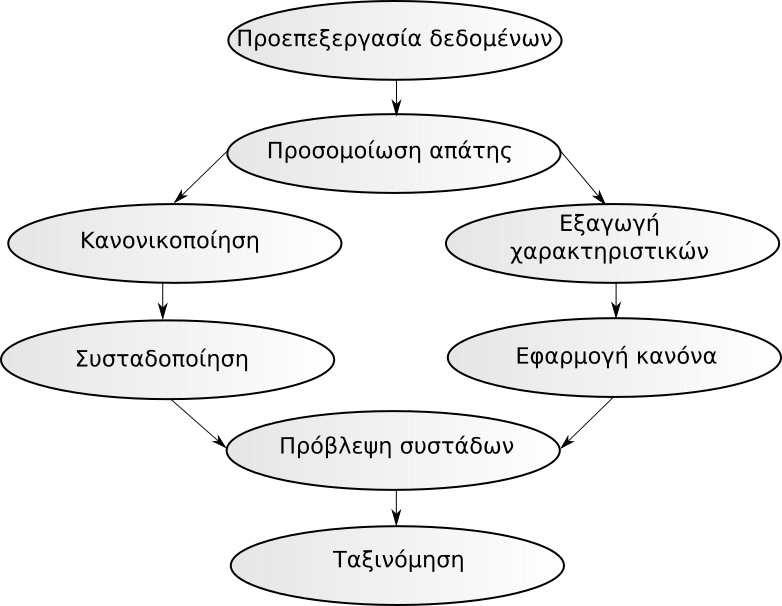
\includegraphics[width=90mm, height=100mm]{../../plots/systems/un_supervised.png}
 \caption{Δομή μη-επιβλεπόμενου ταξινομητή}
\label{fig:unsupervisedsystem}
 \end{figure}
 
\subsection{Εφαρμογή αλγορίθμου συσταδοποίησης}
Η συσταδοποίηση είναι από τους δημοφιλέστερους τύπου μη-επιβλεπόμενης εκμάθησης. Σε αυτό τον τύπο εκμάθησης, ο στόχος δεν είναι η μεγιστοποίηση μιας συνάρτησης, αλλά είναι απλώς η εύρεση των ομοιοτήτων των δεδομένων. Η υπόθεση είναι συνήθως πως οι συστάδες που ανακαλύπτονται θα ταιριάξουν σχετικά καλά με τη διαισθητική ταξινόμηση \cite{aihorizon}.
\subsection{Μεθοδολογία εξαγωγής αποτελεσμάτων}
\section{Δοκιμή αλγορίθμου μη επιβλεπόμενης μάθησης}
\subsection{Αποτελέσματα δοκιμής αλγορίθμου}
\section{Συστατικά αλγορίθμου ημι-επιβλεπόμενης μάθησης}
\subsection{Εφαρμογή αλγορίθμου συσταδοποίησης}
\subsection{Εφαρμογή αλγορίθμου μείωσης διάστασης}
\subsection{Εφαρμογή αλγορίθμου ανίχνευσης ανωμαλιών}
\subsection{Μεθοδολογία εξαγωγής αποτελεσμάτων}
\section{Δοκιμή αλγορίθμου ημι-επιβλεπόμενης μάθησης}
\subsection{Αποτελέσματα δοκιμής αλγορίθμου}
\section{Σχόλια}